

\chapter{Test d'une annexe} 


\section{Première Section de l'Annexe}


\subsection{Figures en annexe}

\begin{figure}
	\centering
	\fbox{
		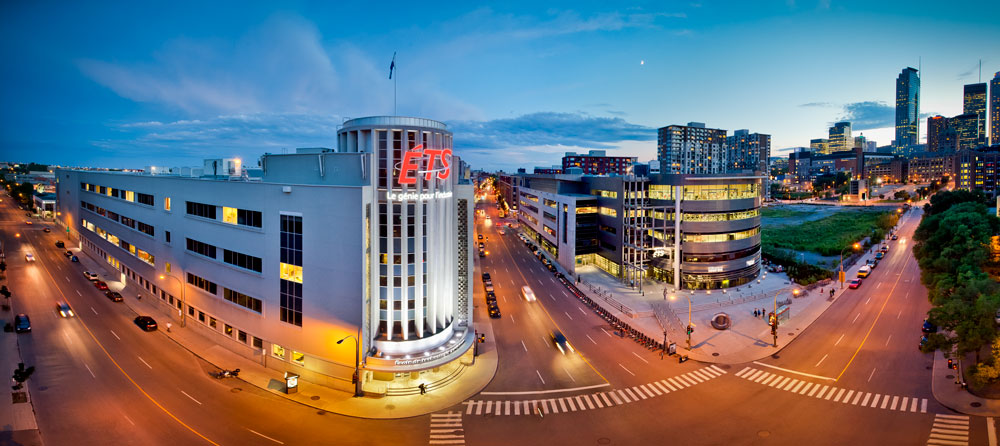
\includegraphics[width=0.75\textwidth]{figures/vueEts.jpg}
	}
	 \\ \parbox{0.75\textwidth}{\caption{Figure en Annexe.}\label{fig:testAp}}
\end{figure}

Les figures en annexe se déclarent de la même manière que dans le reste du document, et leur numération est automatiquement adaptée (exemple, Figure \ref{fig:testAp}).

\subsubsection{Tables en annexe}

\begin{table}
		\parbox{0.65\textwidth}{\caption{Table en Annexe.}\label{tab:testAp}}

		\begin{tabular}{|c|c|c|c|c|c|c|c|}
		\hline
			{\bf titre} & {\bf titre} & {\bf titre} & {\bf titre} & {\bf titre} & {\bf titre} & {\bf titre} & {\bf titre} \\
	  \hline
			blá & blá & blá & blá & blá & blá & blá & blá \\
	  \hline
			blá & blá & blá & blá & blá & blá & blá & blá \\
	  \hline
			blá & blá & blá & blá & blá & blá & blá & blá \\
	  \hline
			blá & blá & blá & blá & blá & blá & blá & blá \\
	  \hline
			blá & blá & blá & blá & blá & blá & blá & blá \\
	  \hline
			blá & blá & blá & blá & blá & blá & blá & blá \\
	  \hline
		\end{tabular}
\end{table}

Même chose pour les tableaux (exemple, Tableau \ref{tab:testAp}).